\documentclass{beamer}
\usepackage{color}
\usepackage{xcolor}
\usepackage[backend=biber]{biblatex}
\usepackage{tikz}
\usepackage{amssymb}
\usepackage[toc]{multitoc}
\usepackage{wrapfig}
\usepackage{subfig}
\usepackage{graphicx}
\usepackage{mathrsfs}
\usepackage{animate}

\renewcommand*{\multicolumntoc}{2}
\setlength{\columnseprule}{1pt}

\setbeamertemplate{bibliography item}{\insertbiblabel}
\AtNextBibliography{\scriptsize}

\RequirePackage{currfile} 
\setbeamertemplate{caption}[numbered]

\usetheme{Frankfurt}
%\usecolortheme{whale}

\addbibresource{main.bib}



%\logo{\includegraphics[width = 0.5 in]{Figures/epscor.jpeg}}

\definecolor{maincol}{HTML}{4B778D}
\definecolor{secondcol}{RGB}{75,119,141}
\definecolor{thirdcol}{RGB}{40,181,181}
\definecolor{orangeCoral}{HTML}{FFC996}
\definecolor{turfGreen}{HTML}{BDD2B6}
\definecolor{algaeRed}{HTML}{CF0000}
\definecolor{parrotBlue}{HTML}{4974A5}
\setbeamercolor{palette primary}{bg = maincol, fg=white}
\setbeamercolor{palette secondary}{bg = secondcol, fg=white}
\setbeamercolor{palette tertiary}{bg=thirdcol, fg=white}
\setbeamercolor{palette quaternary}{bg = thirdcol, fg=white}
\setbeamercolor{structure}{fg=maincol}
\setbeamercolor{section in toc}{fg=maincol} 
\setbeamercolor{subsection in head/foot}{bg=maincol, fg=white}

%--------Stuff for Compartment/Blocks-----%
\usetikzlibrary{arrows}
\tikzstyle{block} = [rectangle, draw, fill=orangeCoral, text width = 1.5em, text centered, minimum height = 2em]
\tikzstyle{blockTurf} = [rectangle, draw, fill=turfGreen!50, text width = 1.5em, text centered, minimum height = 2em]
\tikzstyle{blockAlgae} = [rectangle, draw, fill=algaeRed!45, text width = 1.5em, text centered, minimum height = 2em]
\tikzstyle{blockParrot} = [rectangle, draw, fill=parrotBlue!50, text width = 1.5em, text centered, minimum height = 2em]
\tikzstyle{line} = [thick, ->, >= stealth]
\tikzstyle{dline} = [thick, dashed, ->, >= stealth]
\tikzstyle{noblock} = [rectangle, draw = none]

%%--------------- Title Slide ------------------------------
\title[]{Mathematical Model and Analysis of the Effects of Overfishing on Coral Reef Ecosystems}
\subtitle{Coral Reefsearchers}
\author{Aaron Bumagat, Michelle Luces, Henry Song }
\institute{University of Guam}
\date{\today} 


\begin{document}
\frame{\titlepage}

\AtBeginSection[]{
    \begin{frame}{}
        \frametitle{}
        \setcounter{tocdepth}{2}
        \tableofcontents[currentsection, sections = \thesection]
        \setcounter{tocdepth}{1}
    \end{frame}
}
% \AtBeginSection[]{}
% \begin{frame}<Beamer>
% \frametitle{}
% \setcounter{tocdepth}{2}
% \tableofcontents{currentsection, sections = \thesection}
% \setcounter{tocdepth}{1}
% \end{frame}

%%------------------Table of Contents---------------------------
\begin{frame}{Table of Contents}
    \begin{columns}
        \begin{column}{0.5\textwidth}
            \tableofcontents[sections=1-2]
        \end{column}
        \begin{column}{0.5\textwidth}
            \tableofcontents[sections=3-5]
        \end{column}
    \end{columns}
\end{frame}

%%-----------------------Introduction-------------------------

%%--------------------------Background--------------------------
\section{Background}
\subsection{General Background}
\begin{frame}{Background}
    \begin{itemize}
        \item<1-> Coral Reefs are large underwater structures composed of the skeletons of colonial marine invertebrates known as coral\textsuperscript{\cite{ross}}.
         \item<2-> They play a crucial role in the marine ecosystem's biodiversity along with other functions, such as coastal defense from storms and economic benefits from tourism or local fisheries\textsuperscript{\cite{04_mathanalysis}}.
         \item<3-> According to the 2008 State of the Coral Reef Ecosystems of Guam report, Guam’s coral reef resources are both economically and culturally important, providing numerous goods and services for the residents of Guam, including cultural/traditional use, tourism, recreation, fisheries, and shoreline/infrastructure protection \textsuperscript{\cite{guamwebsite}}.
         \item<4-> Factors that affect coral reefs include climate change, coral reef resilience\textsuperscript{\cite{02_Riegl_Purkis_Model}}, and exploitative fishing practices\textsuperscript{\cite{05_quintero_machuca_cotto_bradley_ríos-soto_2016}}.
    \end{itemize}
\end{frame}

\subsection{General Question}
\begin{frame}{Our Question}
\begin{itemize}
    \item General Question: How will Guam's reef ecosystem change over time?
\end{itemize}
\begin{center}
    $\Downarrow$
\end{center}
\begin{itemize}
    \item Specific Question: How will overfishing affect Guam's coral reef ecosystem over time?
\end{itemize}
\begin{figure}
    \centering
    \includegraphics[width=0.9\textwidth]{Latex/Figures/figure1.png}
    %\caption{Caption}
    %\label{fig:my_label}
\end{figure}
\end{frame}

\subsection{Definitions}
\begin{frame}{Identify Our Terms}
\vspace{-0.2cm}
    \begin{figure}%
        \centering
        \subfloat[\centering Corals\textsuperscript{\cite{img_coral_reef}}]{{\includegraphics[width=4.7cm]{Latex/Figures/coral_reefs.jpg} }}%
        \\
        \subfloat[\centering Algal Turfs\textsuperscript{\cite{img_algal_turf}}]{{\includegraphics[width=3.5cm]{Latex/Figures/algal_turf.jpg} }}%
        \qquad
        \subfloat[\centering Macroalgae\textsuperscript{\cite{img_macroalgae}}]{{\includegraphics[width=3.5cm]{Latex/Figures/macroalgae.jpg} }}%
        \caption{Images of Ecosystem}%
        \label{fig:graphs}%
    \end{figure}
\end{frame}

\begin{frame}{Identify Our Terms (Cont.)}
    \begin{columns}
        \begin{column}{0.5\textwidth}
            \begin{figure}
                \centering
                \includegraphics[width=1\textwidth]{Latex/Figures/parrot_fish.jpg}
                \caption{Parrot Fish\textsuperscript{\cite{img_parrot_fish}}}
                \label{fig:my_label}
            \end{figure}
        \end{column}
        \begin{column}{0.5\textwidth}
            \begin{itemize}
                \item Parrot fish are common reef fish found in many tropical reefs\textsuperscript{\cite{13_blackwood_hastings_mumby_2010}} and are known to feed on algal turfs and macroalgae.
                \item Their bites on corals have been shown to improve and promote coral growth.
                \item Parrot fish are one of the most overfished reef fish in the Caribbean, and potentially on Guam as well\textsuperscript{\cite{13_blackwood_hastings_mumby_2010}}.
            \end{itemize}
        \end{column}
    \end{columns}
\end{frame}


%%------------------------Literature Review----------------
%\section{Literature Rev

    %\begin{itemize}
                %\item Can be used to see which will be focused on when creating our parameters.
            %\end{itemize}
    %\end{itemize}
%\end{frame}

%\begin{frame}{Prioritizing Key Resilience Indicators to Support Coral Reef Management in a Changing Climate Cont.}
%\includegraphics[width = 4.3 in. , height = 1.7 in.]{Figures/Resilience Data.png}
%\end{frame}

%\subsection{Model of coral population response to accelerated bleaching and mass
%mortality in a changing climate}
%\begin{frame}{Model of coral population response to accelerated bleaching and mass mortality in a changing climate}
%    \begin{block}{Summary}
        %Researchers studied coral populations located within the Arabian Peninsula. The study primarily focused on the Porites and %\textit{Acropora} species of coral. The researchers found that coral populations can survive more extreme conditions.
    %\end{block}
%\end{frame}

%\begin{frame}{Model of coral population response to accelerated bleaching and mass
%mortality in a changing climate (Cont.)}
    %Why is this article important?
    %\begin{itemize}
        %\item Methods used include a system of differential equations.
        %\item It implements a compartment model to illustrate the relationships.
        %\item It uses the Lotka-Volterra model to simulate a predator prey relationship between \textit{Acropora} as the dominant species and others as the recessive species.
        %\begin{itemize}
            %\item Incorporates ideas of Game Theory into methods.
        %\end{itemize}
    %\end{itemize}
%\end{frame}

%\subsection{Mathematical Analysis of Coral Reef Models}
%\begin{frame}{Mathematical Analysis of Coral Reef Models}
    %\begin{block}{Summary}
        %This research analyzes grazing in response to threatened coral reef systems. Specifically, this model is focused on the impact of different grazing intensities and their influences on coral-algae interactions. Results provided from this research can provide insight on how to revitalize unhealthy reefs.
    %\end{block}
%\end{frame}

%\begin{frame}{Mathematical Analysis of Coral Reef Models (Cont.)}
    %Why is this article important?
    %\begin{itemize}
        %\item The authors used ordinary differential equations (ODE) and delay differential equations (DDE) to model coral reefs.
        %\item  The mathematical results can help answer how to reverse the unhealthy reefs to a healthy status by knowing how overfishing affects our reefs.
    %\end{itemize}
%\end{frame}

%%------------------------------------------------------


%%-----------------------------Math-------------------------
\section{Mathematical Model} % & Analysis
\subsection{Assumptions}
\begin{frame}{Assumptions}
    \begin{itemize}
        \item Ecosystem:
        \begin{itemize}
            \item is closed (i.e. no migration).
            \item consists of only corals (C), algal turfs (T), and macroalgae (M).
            \item supports maximum carrying capacity of parrotfish.
        \end{itemize}
        \item Macroalgae is the only predator of corals.
        \item Coral recruit to and overgrow algal turfs\textsuperscript{\cite{04_mathanalysis}}.
        \item Corals are overgrown by macroalgae\textsuperscript{\cite{04_mathanalysis}}.
        \item Macroalgae colonize dead coral by spreading vegetative over algal turfs\textsuperscript{\cite{04_mathanalysis}}.
        \item Corals do not naturally die.
        % \item Macroalgae is the only predator for Coral.
        % \item Rates are measured in year(s).
        % \item Coral recruit to and overgrow Algal Turfs\textsuperscript{\cite{04_mathanalysis}}.
        % \item Corals are overgrown by Macroalgae\textsuperscript{\cite{04_mathanalysis}}.
        % \item Macroalgae colonize dead Coral by spreading vegetative over algal turfs\textsuperscript{\cite{04_mathanalysis}}.
        % \item Coral natural death rate is nonexistent (i.e. not from Macroalgae overgrowth).
        % \item Algal turf and macroalgae do not have a death rate.
    \end{itemize}
\end{frame}

\subsection{Compartments}
\begin{frame}{Coral Reef Ecosystem Model Compartments}
    \begin{block}{Compartments}
    The Ecosystem Model consists of 4 compartments:
        \begin{itemize}
        \item \small{$C$: Corals}
        \item \small{$T$: Algal Turfs}
        \item \small{$M$: Macroalgae}
        \item \small{$P$: Parrotfish}
        \end{itemize}
        $$ \text{where } C + T + M = 1.$$
    \end{block}
\end{frame}

\subsection{Parameters}
\begin{frame}{Coral Reef Ecosystem Model Parameters}
\scalebox{0.9}{\begin{minipage}{1.20\textwidth}
\begin{table}
    \centering
    \hspace{-0.7cm}
    \begin{tabular}{c p{5cm} c c}
        \hline
        Parameter & Description & Rate & Units\textsuperscript{\cite{12_noaa_report}\cite{04_mathanalysis}\cite{13_blackwood_hastings_mumby_2010}}\\
        \hline
        \hline
        $\mu_{1}$ & death rate of coral reefs & \colorbox{yellow}{0.15}\textsuperscript{\cite{16_wolanski_richmond_mccook_2004}} & $year^{-1}$\\ %12
        $\mu_{2}$ & natural death rate of parrotfish & \colorbox{yellow}{0.22}\textsuperscript{\cite{12_noaa_report}} & $year^{-1}$\\ %8
        $r$ & rate that coral recruit to overgrow algal turfs & \colorbox{yellow}{10}\textsuperscript{\cite{16_wolanski_richmond_mccook_2004}} & $year^{-1}$\\ %12
        %$g$ & grazing rate that parrotfish graze macroalgae without distinction from algae turfs & $\frac{kg}{yrs}$\\
        $\phi$ & rate that macroalgae spread vegetative over algal turfs & 0.8\textsuperscript{\cite{04_mathanalysis}} & $year^{-1}$\\ %13
        $q$ & intrinsic growth rate for parrotfish & \colorbox{yellow}{0.47}\textsuperscript{\cite{12_noaa_report}} & $year^{-1}$\\ %8
        $h$ & harvesting rate for parrotfish & \colorbox{yellow}{0.14}\textsuperscript{\cite{12_noaa_report}} & $year^{-1}$\\ %8
        $\sigma$ & rate that parrot fish bite coral & 0.01*& $bites \cdot year^{-1}$\\
        $\omega$ & maximum grazing intensity & 1\textsuperscript{\cite{13_blackwood_hastings_mumby_2010}} & -\\
        $\beta$ & carrying capacity of parrotfish & 1 & -\\
        $a_{0}$ & control variable to simulate seasonal changes & 0.99 & - %13
    \end{tabular}
    %\caption{Model Parameters}
    %\label{tab:my_label}
    
\end{table}
\small{* = \textit{estimated value}}\\
\small{\colorbox{yellow}{\#} = \textit{Guam Data}}
\end{minipage}}

% \hspace{-7cm}
%     \begin{table}
%     %\centering
%     \vspace{-1cm}
%     \begin{tabular}{c p{5cm} c c}
%         \hline
%         Parameter & Description & Rate & Units\textsuperscript{\cite{12_noaa_report}\cite{04_mathanalysis}\cite{13_blackwood_hastings_mumby_2010}}\\
%         \hline
%         \hline
%         $\mu_{1}$ & death rate of coral reefs & \colorbox{yellow}{0.15}\textsuperscript{\cite{16_wolanski_richmond_mccook_2004}} & $year^{-1}$\\ %12
%         $\mu_{2}$ & natural death rate of parrotfish & \colorbox{yellow}{0.22}\textsuperscript{\cite{12_noaa_report}} & $year^{-1}$\\ %8
%         $r$ & rate that coral recruit to overgrow algal turfs & \colorbox{yellow}{10}\textsuperscript{\cite{16_wolanski_richmond_mccook_2004}} & $year^{-1}$\\ %12
%         %$g$ & grazing rate that parrotfish graze macroalgae without distinction from algae turfs & $\frac{kg}{yrs}$\\
%         $\phi$ & rate that macroalgae spread vegetative over algal turfs & 0.8\textsuperscript{\cite{11_zikkah_anggriani_supriatna_2020}} & $year^{-1}$\\ %13
%         $q$ & intrinsic growth rate for parrotfish & \colorbox{yellow}{0.47}\textsuperscript{\cite{12_noaa_report}} & $year^{-1}$\\ %8
%         $h$ & harvesting rate for parrotfish & \colorbox{yellow}{0.14}\textsuperscript{\cite{12_noaa_report}} & $year^{-1}$\\ %8
%         $\sigma$ & rate that parrot fish bite coral & 0.01*& $bites \cdot year^{-1}$\\
%         $\omega$ & maximum grazing intensity & 1\textsuperscript{\cite{13_blackwood_hastings_mumby_2010}} & -\\
%         $\beta$ & carrying capacity of parrotfish & 1 & -\\
%         $a_{0}$ & control variable to simulate seasonal changes & 0.99 & - %13
%     \end{tabular}
%     %\caption{Model Parameters}
%     %\label{tab:my_label}
% \end{table}
% * = \textit{estimated value}\\
% \colorbox{yellow}{#} = \textit{Guam Data}
% highlighted values are Guam data
\end{frame}

\subsection{Compartment Model}
\begin{frame}{Coral Reef Ecosystem Model\textsuperscript{\cite{04_mathanalysis}}}
\begin{center}
    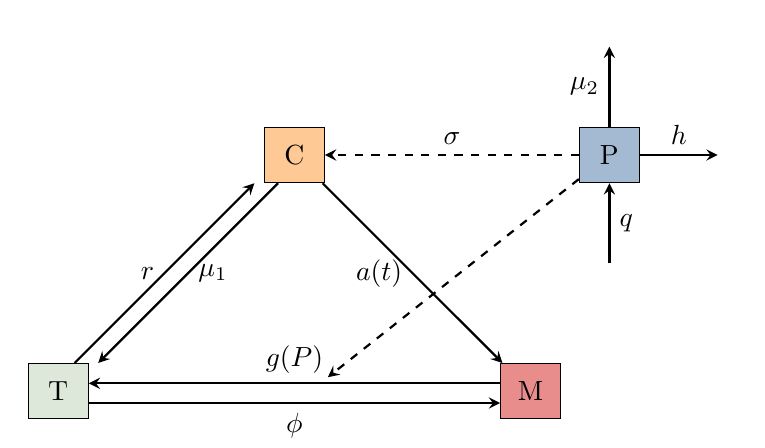
\begin{tikzpicture}{node distance = 1cm, auto}
        \node(leftofC) [noblock] {}; 
        \node(C) [block, right of = leftofC, node distance = 1.5 cm] {C};
        \node(P) [blockParrot, right of = C, node distance = 4 cm] {P};
        \node(belowofC) [noblock, below of = C, node distance = 3 cm]{};
        \node(M) [blockAlgae, right of = belowofC, node distance = 3 cm] {M};
        \node(T) [blockTurf, left of = belowofC, node distance = 3 cm] {T};
        \node(rightofP) [noblock, right of = P, node distance = 1.5 cm]{};
        \node(aboveofP) [noblock, above of = P, node distance = 1.5 cm]{};
        \node(aboveofC) [noblock, above of = C, node distance = 1.5 cm]{};
        \node(belowofP) [noblock, below of = P, node distance = 1.5 cm]{};
        \node(aboveofT) [noblock, above of = T, node distance = 0.08 cm]{};
        \node(diagonalofT) [noblock, right of = aboveofT, node distance = 3.3 cm]{};
        \draw[dline] (P) --node[above]{} (diagonalofT);
        \draw[dline] (P) --node[above]{$\sigma$} (C);
        \draw[line] (C) --node[left]{$a(t)$} (M);
        \draw[line] (P) --node[above]{$h$} (rightofP);
        \draw[line] (P) --node[left]{$\mu_{2}$} (aboveofP);
        %\draw[line] (C) --node[left]{$d$} (aboveofC);
        \draw[line] (belowofP) --node[right]{$q$} (P);
        \begin{scope}[transform canvas = {xshift = -.15cm}]
            \draw[line](T) -- node[left]{$r$} (C);
        \end{scope}
        \begin{scope}[transform canvas = {xshift = .15cm}]
            \draw[line](C) --node[right]{$\mu_{1}$} (T);     
        \end{scope}
        \begin{scope}[transform canvas = {yshift = .1cm}]
            \draw[line] (M) --node[above]{$g(P)$} (T);
        \end{scope}
        \begin{scope}[transform canvas = {yshift = -.15cm}]
            \draw[line] (T) --node[below]{$\phi$} (M);
        \end{scope}
    \end{tikzpicture}
\end{center}
\end{frame}

\subsection{Differential Equations}
\begin{frame}{Differential Equations}
    System of differential equations derived from compartment model:
    \begin{align*}
        \begin{split}
            \frac{dC}{dt} &= rTC + \sigma PC- (a(t)M+\mu_{1})C\\
            \frac{dP}{dt} &= qP \left( 1-\frac{P}{\beta C} \right) - P \left( h+\mu_{2} \right)\\
            \frac{dT}{dt} &= \mu_{1}C + \frac{g(P)M}{M+T} - T(rC+\phi M)\\
            \frac{dM}{dt} &= (a(t)C+ \phi T)M - \frac{g(P)M}{M+T}
            \label{SoODE}
        \end{split}
    \end{align*}
    where $g(P) = \frac{\omega P}{\beta}, \quad a(t)=|\frac{a_{0}(9\sin{(\pi t) }+1)}{10}|$.\\ 
    \quad
    \begin{center}
        {\small \textit{Modified from \cite{13_blackwood_hastings_mumby_2010}}}
    \end{center}
\end{frame}

\subsection{Plots}
\begin{frame}{Simulating $a(t)$}
    \vspace{-1cm}
    \begin{center}
        $$a(t)= \left|\frac{a_{0}(9\sin{(\pi t) }+1)}{10} \right|$$\\
        \animategraphics[width=0.85\textwidth, loop, autoplay]{12}{Latex/Figures/sine_graph_animation/frame-}{157}{318} \\
        \vspace{0.5cm}
        \textit{Plotted using Desmos}
    \end{center}
    
\end{frame}

\begin{frame}{Parameter Changes: $a_{0}$}
    \begin{center}
        \animategraphics[width=0.85\textwidth, loop, autoplay]{3}{Latex/Figures/a_animation/frame-}{1}{45}\\
        Initial Conditions: $C = T = M = \frac{1}{3}$, and $P = \frac{3}{4}$
    \end{center}
\end{frame}

\begin{frame}{Parameter Changes: $h$}
    \begin{center}
        \animategraphics[width=0.85\textwidth, loop, autoplay]{3}{Latex/Figures/h_animation/frame-}{1}{49}\\
        Initial Conditions: $C = T = M = \frac{1}{3}$, and $P = \frac{3}{4}$
    \end{center}
\end{frame}

% \begin{frame}{Parameter Changes: $r$}
%     \begin{center}
%         \animategraphics[width=0.85\textwidth, loop, autoplay]{3}{Latex/Figures/r_animation/Frame-}{1}{49}\\
%         Initial Conditions: $C = T = M = \frac{1}{3}$, and $P = \frac{3}{4}$
%     \end{center}
% \end{frame}

\begin{frame}{Parameter Changes: $\phi$}
    \begin{center}
        \animategraphics[width=0.85\textwidth, loop, autoplay]{3}{Latex/Figures/phi_animation/Frame-}{1}{49}\\
        Initial Conditions: $M = \frac{1}{2}$, $C = T = \frac{1}{4}$, and $P = \frac{3}{4}$
    \end{center}
\end{frame}

\begin{frame}{Compartment Initial Condition Changes}
    \begin{figure}
        \centering
        \includegraphics[width=0.85\textwidth]{Latex/Figures/Graphs/0.3C_0.3T_0.3M.png}
        \caption{Initial Conditions: $C = T = M = \frac{1}{3}$, and $P = \frac{3}{4}$}
        \label{fig:initial_plot}
    \end{figure}
\end{frame}

\begin{frame}{Compartment Initial Condition Changes}
    \begin{figure}
        \centering
        \includegraphics[width=0.85\textwidth]{Latex/Figures/Graphs/0.5C_0.25T_0.25M.png}
        \caption{Initial Conditions: $C = \frac{1}{2}$, $T = M = \frac{1}{4}$, and $P = \frac{3}{4}$}
        \label{fig:coral_dominant}
    \end{figure}
\end{frame}

\begin{frame}{Compartment Initial Condition Changes}
    \begin{figure}
        \centering
        \includegraphics[width=0.85\textwidth]{Latex/Figures/Graphs/0.25C_0.5T_0.25M.png}
        \caption{Initial Conditions: $T = \frac{1}{2}$, $C = M = \frac{1}{4}$, and $P = \frac{3}{4}$}
        \label{fig:turf_dominant}
    \end{figure}
\end{frame}

\begin{frame}{Compartment Initial Condition Changes}
    \begin{figure}
        \centering
        \includegraphics[width=0.85\textwidth]{Latex/Figures/Graphs/0.25C_0.25T_0.5M.png}
        \caption{Initial Conditions: $M = \frac{1}{2}$, $C = T = \frac{1}{4}$, and $P = \frac{3}{4}$}
        \label{fig:macroalgae_dominant}
    \end{figure}
\end{frame}

\section{Equilibria}
\subsection{Disease Free Equilibrium}
\begin{frame}{Disease Free Equilibrium (DFE)}
    \begin{align*}
        C^{0} &= 1 - \frac{\mu_{1}}{r}\\
        P^{0} &= -\frac{\beta(1 - \frac{\mu_{1}}{r})(h - \mu_{2} - q)}{q}\\
        T^{0} &= \frac{\mu_{1}}{r}\\
        M^{0} &= 0 \Longleftarrow \text{our "disease" compartment}
    \end{align*}
    \begin{block}{Note}
    Since C + T + M = 1, if $M^{0} = 0$, then $C^{0} + T^{0} = 1$.
    \end{block}
\end{frame}

\subsection{Endemic Equilibrium}
\begin{frame}{Endemic Equilibrium}
    \scalebox{0.9}{\parbox{.5\textwidth}{%
    \begin{align*}
        T^{*} &= \frac{\mu_{1} + a(t)M^{*}}{r} \\
        &\\
        C^{*} %&= 1-(T^{*} + M^{*}) \\
        &= 1- \left(\frac{\mu_{1} + a(t)M^{*}}{r} + M^{*} \right)\\
        &\\
        P^{*} %&= \beta C^{*} \left(\frac{q-(h+\mu_{2})}{q} \right) \\
        &= \beta \left(1- \left(\frac{\mu_{1} + a(t)M^{*}}{r} + M^{*} \right) \right) \left(\frac{q-(h+\mu_{2})}{q} \right)\\
    %M^{*} &= \frac{\omega (\beta \left(1- \left(\frac{\mu_{1} + a(t)M^{*}}{r} + M^{*} \right) \right) \left(\frac{q-(h+\mu_{2})}{q} \right))}{\beta(a(t)(1- \left(\frac{\mu_{1} + a(t)M^{*}}{r} + M^{*}) \right)+\phi \frac{\mu_{1} + a(t)M^{*}}{r})} - \frac{\mu_{1} + a(t)M^{*}}{r} \\
    \end{align*}
    }}
\end{frame}


\begin{frame}{Endemic Equilibrium Cont.}
Calculation for $M^{*}$:\\
\begin{equation*}
    \frac{-e \pm \sqrt{e^2 - 4df}}{2d}
\end{equation*}
where
\begin{multline*}
    d = (a(t)q-2a(t)r+r \phi ) - q(r^{2}+a(t)^{3})\\
\end{multline*}
\vspace{-1.5cm}
\begin{multline*}
    e = a(t)q(r(r-2\mu_{1}+a(t))-2\mu_{1}(a(t)+\phi )) \\
    + r(q(\phi \mu_{1} + r \omega ) - \omega(hr+a(t) \mu_{2} + r\mu_{2})
\end{multline*}
\vspace{-1cm}
\begin{multline*}
    f = -qr^{2} \omega +qr\mu_{1} \omega + hr^{2} \omega - hr\mu_{1} \omega + r^2 \mu_{2} \omega\\
    - r \mu_{1} \mu_{2} \omega + a(t)qr \mu_{1} -  a(t)q\mu_{1}^{2} +q\phi \mu_{1}^{2}
\end{multline*}
% \begin{align*}
%     d &= (a(t)q-2a(t)r+r \phi ) - q(r^{2}+a(t)^{3})\\
%     e &= a(t)q(r(r-2\mu_{1}+a(t))-2\mu_{1}(a(t)+\phi ))
%     + r(q(\phi \mu_{1} + r \omega ) -   \omega(hr+a(t) \mu_{2} + r\mu_{2})\\
%     f &= -qr^{2} \omega +qr\mu_{1} \omega + hr^{2} \omega - hr\mu_{1} \omega + r^2 \mu_{2} \omega - r \mu_{1} \mu_{2} \omega + a(t)qr \mu_{1} -  a(t)q\mu_{1}^{2} +q\phi \mu_{1}^{2}
% \end{align*}

\end{frame}

\subsection{Basic Reproduction Number}
\begin{frame}{Basic Reproduction Number: $\mathscr{R}_{0}$}
    \begin{block}{Definition}
        \begin{itemize}
            \item A metric used to describe the contagiousness or transmissibility of infectious agents\textsuperscript{\cite{delamater_street_leslie_yang_jacobsen_2019}}, i.e. the number of secondary infections. % general def
            \item $\mathscr{R}_{0}$ is the rate at which macroalgae spreads after the initial macroalgae overgrowth. % def in terms of our model
        \end{itemize}
        
    \end{block}
\end{frame}

\begin{frame}{Basic Reproduction Number: $\mathscr{R}_{0}$}
    \begin{columns}
        \begin{column}{0.5\textwidth}
            \begin{align*}
                \mathscr{F} &= \begin{bmatrix} a(t)CM+\phi TM \end{bmatrix}\\
                \Downarrow\\
                F &= \begin{bmatrix} a(t)C^{0} + \phi T^{0} \end{bmatrix}
            \end{align*}
        \end{column}
        \begin{column}{0.5\textwidth}
            \begin{align*}
                \mathscr{V} &= \begin{bmatrix} \frac{g(P)M}{M+T} \end{bmatrix}\\
                \Downarrow\\
                V &= \begin{bmatrix} \frac{g(P)T^{0}}{(M^{0}+T^{0})^{2}} \end{bmatrix}
            \end{align*}
        \end{column}
    \end{columns}
    $$\mathscr{R}_{0} = \rho(\det(FV^{-1} - \lambda I))$$
    $$\Downarrow$$
    \centering
    $\displaystyle {\mathscr{R}}_{0} = - \frac{\beta \mu_{1}q(a(t)(\frac{\mu_{1}}{r}-1)-\frac{\mu_{1}}{r})}{\omega r (\beta h (\frac{\mu_{1}}{r}-1) + \beta \mu_{2} (\frac{\mu_{1}}{r}-1) - \beta q(\frac{\mu_{1}}{r}-1))}$
\end{frame}

\subsection{Sensitivity Analysis}
\begin{frame}{Sensitivity Analysis for $\mathscr{R}_0$}
    \begin{columns}
        \begin{column}{0.6\textwidth}
        \small
            % \begin{block}{Sensitivity Analysis for $\mathscr{R}_0$}
            The Sensitivity Analysis for $\mathscr{R}_0$ determines the most influential parameters affecting $\mathscr{R}_0$. It is defined by
                $$S_{\lambda} = \frac{\frac{\Delta \mathscr{R}_{0}}{\mathscr{R}_{0}}}{\frac{\Delta x}{x}} = \frac{\lambda}{\mathscr{R}_{0}} \cdot \frac{\partial \mathscr{R}_{0}}{\partial \lambda}$$ \\
                where $\lambda$ is a parameter in the quantity $\mathscr{R}_{0}$
            % \end{block} 
        \end{column}
        \begin{column}{0.4\textwidth}
            \begin{table}[H]
                \centering
                \begin{tabular}{|c|c|}
                \hline
                    $\lambda$ & $S_{\lambda}$ \\
                    \hline
                    \hline
                    $\mu_{1}$ & \colorbox{yellow}{\textbf{8.3513}}\\
                    \hline
                    $\mu_{2}$ & \colorbox{yellow}{\textbf{5.2819}}\\
                    \hline
                    $q$ & -3.5962\\
                    \hline
                    $\omega$ & -0.7923\\
                    \hline
                    $\sigma$ & 0\\
                    \hline
                    $r$ & -2.5054\\
                    \hline
                    $\phi$ & 0.4029\\
                    \hline
                    $\beta$ & 0\\
                    \hline
                    $h$ & \colorbox{yellow}{\textbf{5.2819}}\\
                    \hline
                    $a(t)$ & 0.94\\
                    \hline
                \end{tabular}
                \caption{Sensitivity Analysis}
                \label{tab:sens_analysis}
            \end{table}
        \end{column}
    \end{columns}
\end{frame}

\begin{frame}{Sensitivity Analysis for $\mathscr{R}_{0}^{\mu_1}$}
    \begin{figure}
        \centering
        \includegraphics[width=0.8\textwidth]{Latex/Figures/Graphs/mu1_sens_analysis.png}
        \caption{Effects of various $\mu_{1}$ values on $\mathscr{R}_{0}$}
        \label{fig:mu1_sens_analysis}
    \end{figure}
\end{frame}



\section{Harvesting Game Theory}

\begin{frame}{Harvesting Game}
Game of Harvesting 
\begin{itemize}
    \item \textbf{Player:} Individual
    \item \textbf{Strategy: } 
        \begin{itemize}
            \item Proportion of Individual Harvesting ($h$) based on the rate the population is harvesting ($h_{pop}$)
        \end{itemize}
\end{itemize}
\end{frame}

\subsection{Harvesting Threshold}
\begin{frame}{Harvesting Threshold}
    \begin{block}{Definition (Harvesting Threshold)}
        The rate at which parrotfish can be harvested in order for macroalgae growth to become stable in the ecosystem. 
    \end{block}
    
    \vspace{0.5cm}
    
    When $\mathscr{R}_{0} = 1$,
    \begin{center}
    
    $\displaystyle{h_{TH} = q - \mu_{2} + \frac{\mu_{1}q(a(t) \mu_{1} - a(t)r - \phi \mu_{1})}{\omega r(r-\mu_{1})}}$ \\
    \end{center}
    \begin{align*}
    h_{pop} &< h_{TH}: \text{Macroalgae growth is stable} \\
    h_{pop} &> h_{TH}: \text{Macroalgae growth is unstable}
    \end{align*}
\end{frame}

\begin{frame}{Harvesting Threshold Graph}
    \begin{figure}
        \centering
        \includegraphics[width = 0.85\textwidth]{Latex/Figures/Graphs/threshold_graph.png}
        \caption{When $\mathscr{R}_0 = 1$, $h = 0.1312$}
        \label{fig:threshold}
    \end{figure}
\end{frame}

\subsection{Expected Payoff - Harvesting}
\begin{frame}{Expected Payoff - Harvesting}
    Let h $\in$ [0,1] be the proportion at which an individual can harvest parrotfish.
    \begin{center}
    $\displaystyle {E(h, h_{pop}) = -hC_{h} - \left( \frac{h_{pop}}{h_{pop} + \mu_{2}} \cdot \frac{g(P^{*})(1-h)M^{*}}{M^{*} + T^{*}} \right) C_{D}}$ \\
    
    \vspace{0.6cm}
    
    \begin{table}[H]
        \centering
        \begin{tabular}{c|p{8cm}}
             Symbol & Definition \\
             \hline
             $E(h, h_{pop})$ & Expected payoff for an individual to harvest based on the harvesting rate of the population \\
             $C_{h}$ & Cost of harvesting \\
             $C_{D}$ & Cost of coral disease \\
        \end{tabular}
        %\caption{Caption}
        \label{tab:my_label}
    \end{table}
    \end{center}
\end{frame}

\begin{frame}{Expected Payoff - Harvesting}
    \begin{center}
    $\displaystyle {E(h, h_{pop}) = -hC^{h} - \frac{h_{pop}}{h_{pop} + \mu_{2}} \cdot \frac{g(P^{*})(1-h)M^{*}}{M^{*} + T^{*}}}$ \\
    
    \vspace{0.6cm}
    
    where $C^{h} = \frac{C_{h}}{C_{D}}$
    \end{center}
\end{frame}

\begin{frame}{Expected Payoff - Harvesting}

$E(h, h_{pop})$ is a convex function since 
$\frac{\partial^{2}E(h, h_{pop})}{\partial h^{2}} > 0$ \\

$$\displaystyle {\frac{\partial ^ {2} E}{\partial h^{2}} = \frac{2 \omega P \mu{2} (M^{*}+T^{*})^{2} (\mu_{1} +1)}{\beta(h(M^{*}+T^{*}) + \mu_{2}(M^{*}+T^{*}))^{3}} > 0}$$
\vspace{0.6cm}

Thus, $E$ achieves a maximum value at $h = 0$ or $h=1$.

\end{frame}

\subsection{Nash Equilibrium}
\begin{frame}{What is Nash Equilibrium?}
    \begin{block}{Definition\textsuperscript{\cite{nash_definition}}}
        \begin{itemize}
            \item The \textbf{Nash equilibrium} is a decision-making theorem within game theory that states a player can achieve the desired outcome by not deviating from their initial strategy.
            \item Each player's strategy is optimal when considering the decisions of other players. Every player wins because everyone gets the outcome they desire.
            %\item A common Nash equilibrium problem is the prisoner's dilemma game.
        \end{itemize}
    \end{block}
\end{frame}

\begin{frame}{Nash Equilibrium - Harvesting}
    To obtain the Nash Equilibrium, we let $E(0, h_{pop}) = E(1, h_{pop})$, where \\
    \begin{align*}
        E(0, h_{pop}) &= -\frac{h_{pop}}{h_{pop} + \mu_{2}} \cdot \frac{g(P^{*})M^{*}}{M^{*} + T^{*}} \\
        E(1, h_{pop}) &= -C^{h}
    \end{align*}
    $$\Downarrow$$
    
    $$\frac{h_{pop}}{h_{pop} + \mu_{2}} \cdot \frac{g(P^{*})M^{*}}{M^{*} + T^{*}} = C^{h}$$

\end{frame}
            

\begin{frame}{Nash Equilibrium Graph}
    \begin{columns}
        \begin{column}{0.7\textwidth}
            \hspace{0.5cm}
            \begin{figure}
                \centering
                \includegraphics[width = \textwidth]{Latex/Figures/Graphs/nash_1.png}
                \caption{Nash Equilibrium Graph}
                \label{fig:NE_Graph}
            \end{figure}
        \end{column}
        \begin{column}{0.2\textwidth}
            \hspace{-1.3cm}
            \begin{align*}
                %h &= equation\\
                \Delta E &= E(1, h_{pop}) - E(0, h_{pop}) \\
                \Delta E &< 0: \text{Harvest} \\
                \Delta E &> 0: \text{Do Not Harvest}
            \end{align*}
        \end{column}
    \end{columns}
\end{frame}


%----------------------------------------------------

%---------------------Conclusion---------------------
\section{Discussion}
\begin{frame}{Discussion}
    \begin{itemize}
        \item<1-> Overfishing can have a detrimental impact on coral reef ecosystems.
        \item<2-> Based on our mathematical model:
            \begin{itemize}
                \item A higher $a_{0}$ will result in higher macroalgae growth over corals, especially over warmer months of the year.
                \item A higher $h$ will result in the increased dominance of macroalgae in the ecosystem.
                \item A lower $\phi$ will result in decreased proportion of macroalgae and increase in algal turfs, and subsequently corals.
            \end{itemize}
        \item<3-> Our sensitivity analysis indicates that our coral death rate ($\mu_{1}$), parrotfish natural death rate ($\mu_{2}$), and harvesting rate ($h$) have the largest impact on our basic reproduction number.
    \end{itemize}
\end{frame}

\begin{frame}{Discussion}
    \begin{itemize}
        \item<1-> The maximum harvest rate without cost is approximately 0.131157 (13.1157\%) of the parrot fish population. 
        \item<2-> According to our harvesting game theory, as the relative cost of fishing increases, the harvesting threshold decreases until it reaches the maximum cost.
    \end{itemize}
\end{frame}
%----------------------------------------------------

%---------------------Plans---------------------
\section{Closing Remarks}
\subsection{Future Research}
\begin{frame}{Future Research}
    \begin{itemize}
    \item Find data from Guam sources to give a more accurate representation of the changes on Guam's Reef Ecosystem. 
    \item Application of game theory on $\phi$ parameter control measures.
    \item Incorporate more elements of coral reef ecosystems (i.e. other types of plant and aquatic life) to our compartment model.
        %\item Specific ideas:
        %\begin{itemize}
           % \item How will a specific coral species change throughout the upcoming decades on Guam?
            %\item Select a representative species of average resiliency (specifically on Guam) and examine how it will change over time through climate changes.
        %\end{itemize}
        %\item Continue to digest articles and literature relevant to our research.
        %\item Finish endemic equilibrium calculations.
        %\item Perform sensitivity analysis on parameters.
        %\item Refine and improve differential equations to improve dynamics
        %\item Continue application of Harvesting Game Theory on the harvest rate parameter ($h$) to quantify human behavior and the best strategy to protect coral reef sustainability. These tasks include:
        %\begin{itemize}
            %\item Payoff Matrix
            %\item Dominant and/or mixed equilibrium equations
            %\item continue solving for the Nash Equilibrium %/Evolutionary Stable Strategy
            %\item Replicator Equation
        %\end{itemize}
    \end{itemize} 
\end{frame}

%----------------------------------------------------


\subsection{Q \& A}
\begin{frame}
    \begin{center}
        \Huge{Questions or Comments?}
    \end{center}
\end{frame}

%%-------------------------Acknowledgements----------------
\subsection{Acknowledgements}
\begin{frame}{Acknowledgements}
    \begin{center}
        Support for the Young Scholars Research Experience in Mathematics (YSREM)  is through the MAA Tensor SUMMA Program. Support for the MAA National Research Experience for Undergraduates Program (NREUP) is provided by the National Science Foundation (Grant Number DMS-1950644). Support for the NSF EPSCoR project, Guam Ecosystems Collaboratorium for Corals and Oceans (GECCO) is provided by the National Science Foundation (Grant Number DMS-1946352). \\
    \vspace{.2cm}
    \small{Special thanks to the UOG Marine Laboratory(Dr. Bastian Bentlage and Ms. Grace McDermott), our faculty mentors (Dr. JaeYong Choi, Dr. HyunJu Oh, \& Dr. Leslie Aquino), and our Research Assistants (Jaron Bautista \& Regina-Mae Dominguez).}
    
    \begin{figure}
        \includegraphics[width = 0.20\textwidth]{Figures/MAA_logo_PMS286.jpg}
        \label{MAA}
        \includegraphics[width = 0.12\textwidth]{Figures/NSF_4-Color_bitmap_Logo.png}
        \label{NSF}
        % \includegraphics[width = 0.20\textwidth]{Figures/GECCO.png}
        % \label{gecco}
        \includegraphics[width = 0.12\textwidth]{Figures/epscor.jpeg}
        \label{epscor}
        \includegraphics[width = 0.20\textwidth]{Figures/UOG-horizontal.png}
        \label{uog}
    \end{figure}
    \end{center}
\end{frame}




%%----------------------Bibliography-------------------
\subsection{Bibliography}
\begin{frame}[allowframebreaks]{Bibliography}
    \printbibliography
\end{frame}


%%---------------Thank you/Questions----------------------

\begin{frame}
    \begin{center}
        \Huge{Thank you!}
    \end{center}
\end{frame}


\end{document}